\chapter{Retry}\label{ch:retry}


\section{Introduction}\label{sec:retry-context}

The retry mechanism is a resilience pattern that allows an application to handle transient failures when it tries to connect to a service or network resource.
By transparently retrying a failed operation, the application can improve its stability and availability~\cite{microsoft-retry-pattern}.

This mechanism, as illustrated in Figure~\ref{fig:retry-execution-example}, is particularly useful when the application is interacting with services that are prone to temporary failures, such as network issues, temporary unavailability of services, or timeouts when services are overloaded.
These issues are often brief and resolve themselves within a short period, meaning that retrying the operation after a short delay can often succeed (e.g., a call to a service that is temporarily overloaded might succeed if retried after a few seconds)~\cite{microsoft-retry-pattern}.

Without a retry mechanism, an application might treat such transient failures as critical,
leading to unnecessary disruptions in service, increased latency, and a poor user experience.

When an application detects a failure (e.g., when sending a request to a remote service), it can handle it using the following strategies~\cite{microsoft-retry-pattern}:

\begin{itemize}
    \item \textbf{Cancel}: If the fault indicates that the failure isn't transient or is unlikely to be successful if repeated, the application should cancel the operation and report an exception (e.g., an authentication failure caused by providing invalid credentials is not likely to succeed no matter how many times it's attempted);
    \item \textbf{Retry}: If the specific fault reported is unusual or rare, it might have been caused by unusual circumstances (e.g., a transient network issue).
    In this case, the application could retry the failing request again immediately because the same failure is unlikely to be repeated;
    \item \textbf{Retry after delay}: If the fault is caused by one of the more commonplace connectivity or busy failures, the network or service might need a short period while the connectivity issues are corrected or the backlog of work is cleared.
    The application should wait for a suitable time (wait duration) before retrying the request.
    The amount of time to wait before retrying depends on:
    \begin{itemize}
        \item the type of failure and the probability that it'll be corrected during this time;
        \item the delay strategy used (e.g., constant, linear, exponential);
    \end{itemize}
\end{itemize}

\begin{figure}[!htb]
    \centering
    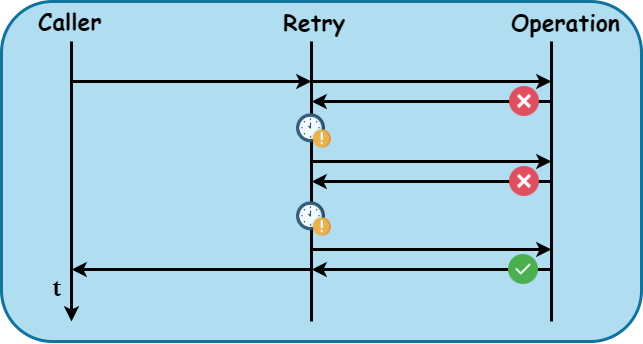
\includegraphics[width=0.6\textwidth]{../figures/04_retry-execution-example}
    \caption{Retry Execution Example}
    \label{fig:retry-execution-example}
\end{figure}

\subsection{Delay Strategies}\label{subsec:retry-delay-strategies}

The retry delay strategy defines the amount of time the application should wait before retrying the operation, and it can be one of the following:

\begin{itemize}
    \item \textbf{No Delay}: This strategy does not introduce any delay between retries;
    \item \textbf{Constant Delay}: Introduces a fixed, constant delay between each retry attempt;
    \item \textbf{Linear Delay}: Increases the delay duration linearly with each retry attempt.
    The delay is calculated by multiplying the initial delay by the retry attempt number (e.g., \texttt{initial delay=1s, retry attempt=4, result=[1, 2, 3, 4]});
    \item \textbf{Exponential Delay}: This strategy exponentially increases the delay duration with each retry attempt, by using the \textit{exponential backoff algorithm}.
    Essentially, the delay is calculated by multiplying the initial delay by a specified multiplier raised to the power of the retry attempt number (e.g., \texttt{initial delay=1s, multiplier=2, retry attempt=4, result=[1, 2, 4, 8]});
    \item \textbf{Custom Delay}: This strategy uses a custom function to calculate the delay duration based on the retry attempt number and the last exception caught (if any), allowing for more complex delay strategies (e.g., a delay that increases linearly for the first 3 attempts, then doubles for the next 3 attempts, and so on).
\end{itemize}

In both linear and exponential delay strategies, a maximum delay can be set to prevent potentially excessive delays caused by the growth of the delay duration with each retry attempt.

Additionally, a \textit{jitter} can be introduced to randomize the calculated delay duration.
This randomization can help
avoid synchronization between multiple clients that are retrying the same operation at the same time,
commonly known as the \textit{thundering herd problem}, by spreading out the retries over a period of time.


\section{Configuration}\label{sec:retry-configuration}

The retry mechanism can be configured using a dedicated configuration builder with the properties listed in Table~\ref{tab:retry-config-builder}.

\begin{table}[!htb]
    \centering
    \caption{Configuration Properties for \texttt{RetryConfigBuilder}}
    \label{tab:retry-config-builder}
    \vspace{0.3cm}
    \begin{tabular}{|l|p{5cm}|p{6cm}|}
        \hline
        \textbf{Config Property}        & \textbf{Default Value/Behaviour}                                       & \textbf{Description}                                                                            \\ \hline
        \texttt{maxAttempts}            & \texttt{3}                                                             & The maximum number of attempts (including the initial call as the first attempt).               \\ \hline
        \texttt{retryPredicate}         & \texttt{throwable -> true}                                             & Predicate to determine if the operation should be retried based on the caught throwable.        \\ \hline
        \texttt{retryOnResultPredicate} & \texttt{result -> false}                                               & Predicate to determine if the operation should be retried based on the result of the operation. \\ \hline
        \texttt{delayStrategy}          & \texttt{Exponential[ initialDelay=500ms, multiplier=2.0, maxDelay=1m]}          & The strategy for calculating delay between retries.                                             \\ \hline
        \texttt{resultMapper} & \texttt{Rethrow throwable
        if any or return result unmodified}          & Function
        to map the result or exception after the retry mechanism cannot be used any more to retry an operation                            \\ \hline
    \end{tabular}
\end{table}

The default configuration can be overriden by calling the respective builder methods.
The values that compose the default configuration are the most common and recommended for most use cases, but they can be adjusted to better suit the application's needs.

\subsection{Custom Delay Provider}\label{subsec:retry-custom-delay-provider}

A custom delay provider can be used
to implement a custom delay strategy that differs from the standard delay strategies (see Section~\ref{subsec:retry-delay-strategies}).

A delay strategy determines the next wait time between retry attempts,
while a delay provider executes the actual waiting period by pausing or blocking
(dependends on the implementation) the process for the specified duration.

For example, for testing purposes, the custom delay provider might be implemented to not delay using real time,
but instead, immediately continue the execution,
and only keeping track of the time that would have been spent waiting (virtual time).
This can be useful for speeding up tests that involve retry mechanisms, as it allows for faster execution without actually waiting for the delay duration.

A custom delay provider also allows maintaining external state
(e.g., additional configuration through other dependencies) that can be used to calculate the delay duration,
which can't be achieved with the standard delay strategies.


\section{Implementation Aspects}\label{sec:retry-implementation-aspects}

TODO: Describe what deviates from the Mechanism model

\subsection{Ignoring Exceptions}\label{subsec:retry-ignoring-exceptions}

The idea of ignoring exceptions that shouldn't trigger a retry was initially considered,
by adding an extra configuration property (as offered by Resilience4j~\cite{resilience4j-retry}).
However, it was decided
that the retry predicate should be the only policy for determining if an operation should be retried based on the caught exception.

\subsection{Result Mapper}\label{subsec:retry-result-mapper}

During the initial development phases, if an operation failed after multiple retries,
the last caught exception was always rethrown,
and the original result was returned without any modifications.
This approach is sufficient for most use cases,
and most studied implementations of the retry mechanism follow this pattern, but
it was decided to provide a more flexible solution
(e.g., the caller doesn't want a specific exception to be thrown, but instead wants to log it only).
To address this, an exception handler was introduced to the configuration.
This handler allowed for additional processing of the caught exception
(e.g., decide if it should be rethrown or logged),
but still did not provide a way to modify the result of the underlying operation.

To provide even more flexibility, a result mapper was subsequently added to the configuration.
This mapper enables customized handling of the result or exception once the retry mechanism could not be used any more,
allowing for more complex scenarios to be managed while keeping the already established functionality intact.
Additionally, the result mapper can be reconfigured per decoration.

\subsection{Retry Context}\label{subsec:retry-context}

The retry context represents the asynchronous context mechanism's model component implementation (see Section~\ref{subsec:asynchronous-context}), which is responsible for managing the state and controlling the flow of retryable operations.
It maintains internal state information, such as the number of retry attempts and the last-caught exception,
and has access to the configuration settings defined for the retry mechanism.
Additionally, it emits events to potential listeners.

In the later stages of development,
the retry context was made available to the operation being retried (see Section~\ref{subsec:operation-context}),
allowing it to access the context and potentially alter its behaviour based on its state.

\subsubsection{Event Emission}\label{subsubsec:retry-context-event-emission}

The retry context emits the following events, when the operation:

\begin{itemize}
    \item has succeeded and the retry mechanism is no longer needed;
    \item is about to be retried;
    \item has failed, and the retry mechanism cannot be used any more.
    Two different event types can be emitted in this case based on if the last-caught exception was expected or not.
\end{itemize}

\subsection{Execution Flow}\label{subsec:retry-execution-flow}

A retry mechanism can be used to decorate an operation.
When the operation is executed, a new retry context is created (per-method invocation).
The outcome of the operation—success or failure—is determined by the policies defined in this configuration.

When the underlying operation is executed, the retry context captures any exception or result that occurs.
If the operation fails,
the retry context consults the policies defined in the configuration to decide if a retry should be attempted.
If so, the operation is repeated after a delay, calculated based on the specified delay strategy.
But if the retry context determines that the operation should not be retried,
the operation is considered to have failed.

If the operation eventually succeeds through the retry mechanism, the retry is considered successful.
In all cases where the retry mechanism cannot be used any more
(e.g., the maximum number of attempts has been reached), the result mapper is called to map the final result or exception before it is returned to the caller.

This description can be visualized in the retry mechanism execution flow, as illustrated in Figure~\ref{fig:retry-execution-flow}.

\begin{figure}[!htb]
    \centering
    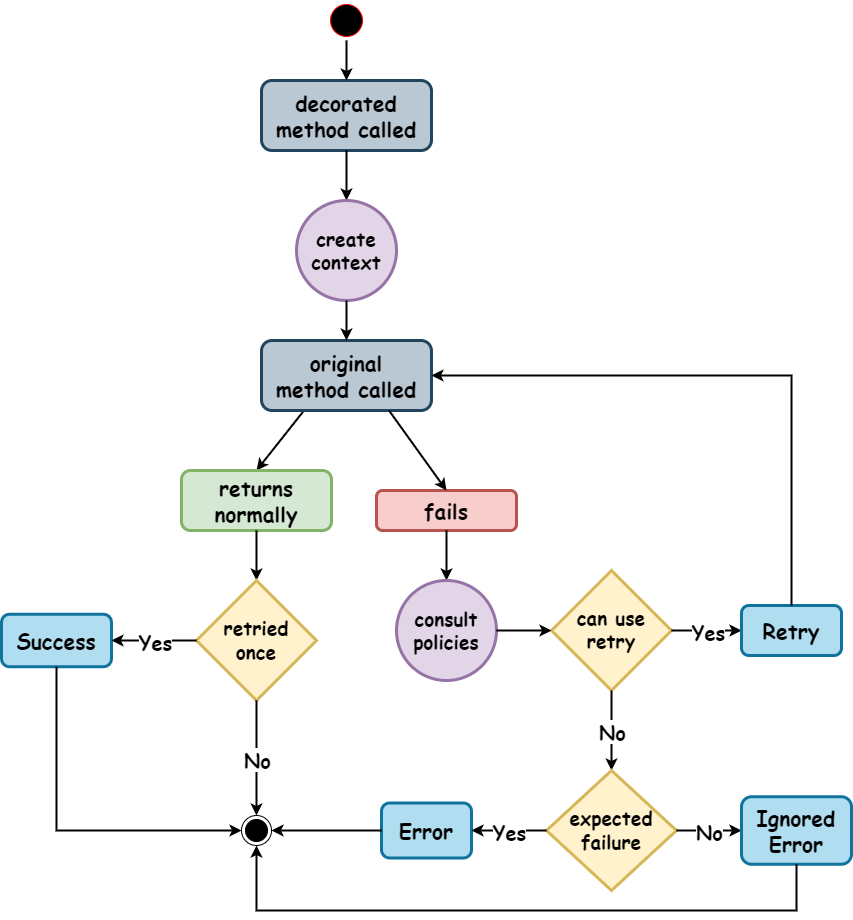
\includegraphics[width=0.6\textwidth]{../figures/04_retry-execution-flow}
    \caption{Retry Mechanism Execution Flow}
    \label{fig:retry-execution-flow}
\end{figure}


\section{Ktor Integration}\label{sec:retry-ktor-integration}

The retry mechanism was integrated with Ktor
by implementing a custom plugin that can be added to the application's Ktor pipeline,
using the implemented retry mechanism.

\subsection{Plugin Implementation}\label{subsec:request-retry-plugin}

The plugin was designed for Ktor clients to enable automatic retries for HTTP requests.
It intercepts the sending phase of a request,
applying configurable retry logic based on conditions such as response status or exceptions.

Before retrying a request,
the plugin copies the original request and propagates its completion state to the copy,
ensuring completion synchronization between the original and the retry request (e.g., if the original request is cancelled, the retry request is also cancelled).

The plugin allows for two levels of configuration:

\begin{itemize}
    \item \textbf{Global Configuration}: The configuration is set during the plugin installation and applies to all requests made by the client;
    \item \textbf{Per-Request Customization}: The configuration can be overridden for a specific request, allowing for more fine-grained control over the retry logic (e.g., disabling the retry mechanism for a specific request).
\end{itemize}

A listener to log all events emitted by the retry context is also enabled, which cancels its subscription when the request is completed.

\subsection{Configuration}\label{subsec:retry-ktor-configuration}

The retry Ktor plugin can be configured by providing a configuration builder with the properties listed in Table~\ref{tab:retry-ktor-config-builder}.

\begin{table}[!htb]
    \centering
    \caption{Configuration Properties for \texttt{RetryPluginConfigBuilder}}
    \label{tab:retry-ktor-config-builder}
    \vspace{0.3cm}
    \begin{tabular}{|l|p{5cm}|p{6cm}|}
        \hline
        \textbf{Config Property}           & \textbf{Default Value/Behaviour}                                                    & \textbf{Description}                                                                                   \\ \hline
        \texttt{maxAttempts}               & \texttt{3}                                                                          & The maximum number of attempts (including the initial call as the first attempt).                      \\ \hline
        \texttt{retryOnExceptionPredicate} & \texttt{throwable -> true}                                                          & Predicate to determine if the operation should be retried based on the caught throwable.               \\ \hline
        \texttt{delayStrategy}             & \texttt{Exponential[ initialDelay=500ms, multiplier=2.0, maxDelay=1m]}          & The strategy for calculating delay between retries.                                             \\ \hline
        \texttt{retryOnCallPredicate}      & \texttt{(request, response) -> retries if a 5xx response is received from a server} & Predicate to determine if an HTTP call should be retried based on the respective request and response. \\ \hline
        \texttt{modifyRequestOnRetry}      & \texttt{(requestBuilder, attempt) -> no-operation} & Callback to modify the request between retries (e.g., add a header with the current attempt number). \\ \hline
    \end{tabular}
\end{table}

Additionally, methods relevant to an HTTP context were added to the configuration builder to simplify the configuration process:

\begin{itemize}
    \item \texttt{retryOnServerErrors}: Retries the HTTP call if the response status code is in the range: 500-599;
    \item \texttt{retryOnServerErrorsIfIdempotent}: Similar to \texttt{retryOnServerErrors}, but only retries if the request method is idempotent~\cite{idempotent-http-method} (e.g., \texttt{GET, PUT, DELETE});
    \item \texttt{retryOnTimeout}: Retries the HTTP call if the exception thrown is a timeout exception (e.g., connection timeout exceeded).
\end{itemize}
